% inkscape sierpinski.pdf --export-type=png --export-filename=sierpinski.png --export-width=1024 --export-background-opacity=0
% \documentclass[a3paper]{article}
% \usepackage[left=0mm,top=1cm,right=0mm,bottom=0mm]{geometry}
\documentclass[border=0]{standalone}
% \documentclass[dvisvgm]{minimal}
\usepackage{tikz}
\usetikzlibrary{calc,lindenmayersystems}
\usepackage{xcolor}
\definecolor{pGreen}{HTML}{663366}
\pgfdeclarelindenmayersystem{Sierpinski Gasket}{
\symbol{F}{\pgflsystemdrawforward}
\symbol{A}{\pgflsystemdrawforward}
\symbol{+}{\pgflsystemturnright} % Explicitly define + and - symbols.
\symbol{-}{\pgflsystemturnleft}
\rule{A -> A-F+A+F-A}
\rule{F -> FF}
}
\begin{document}
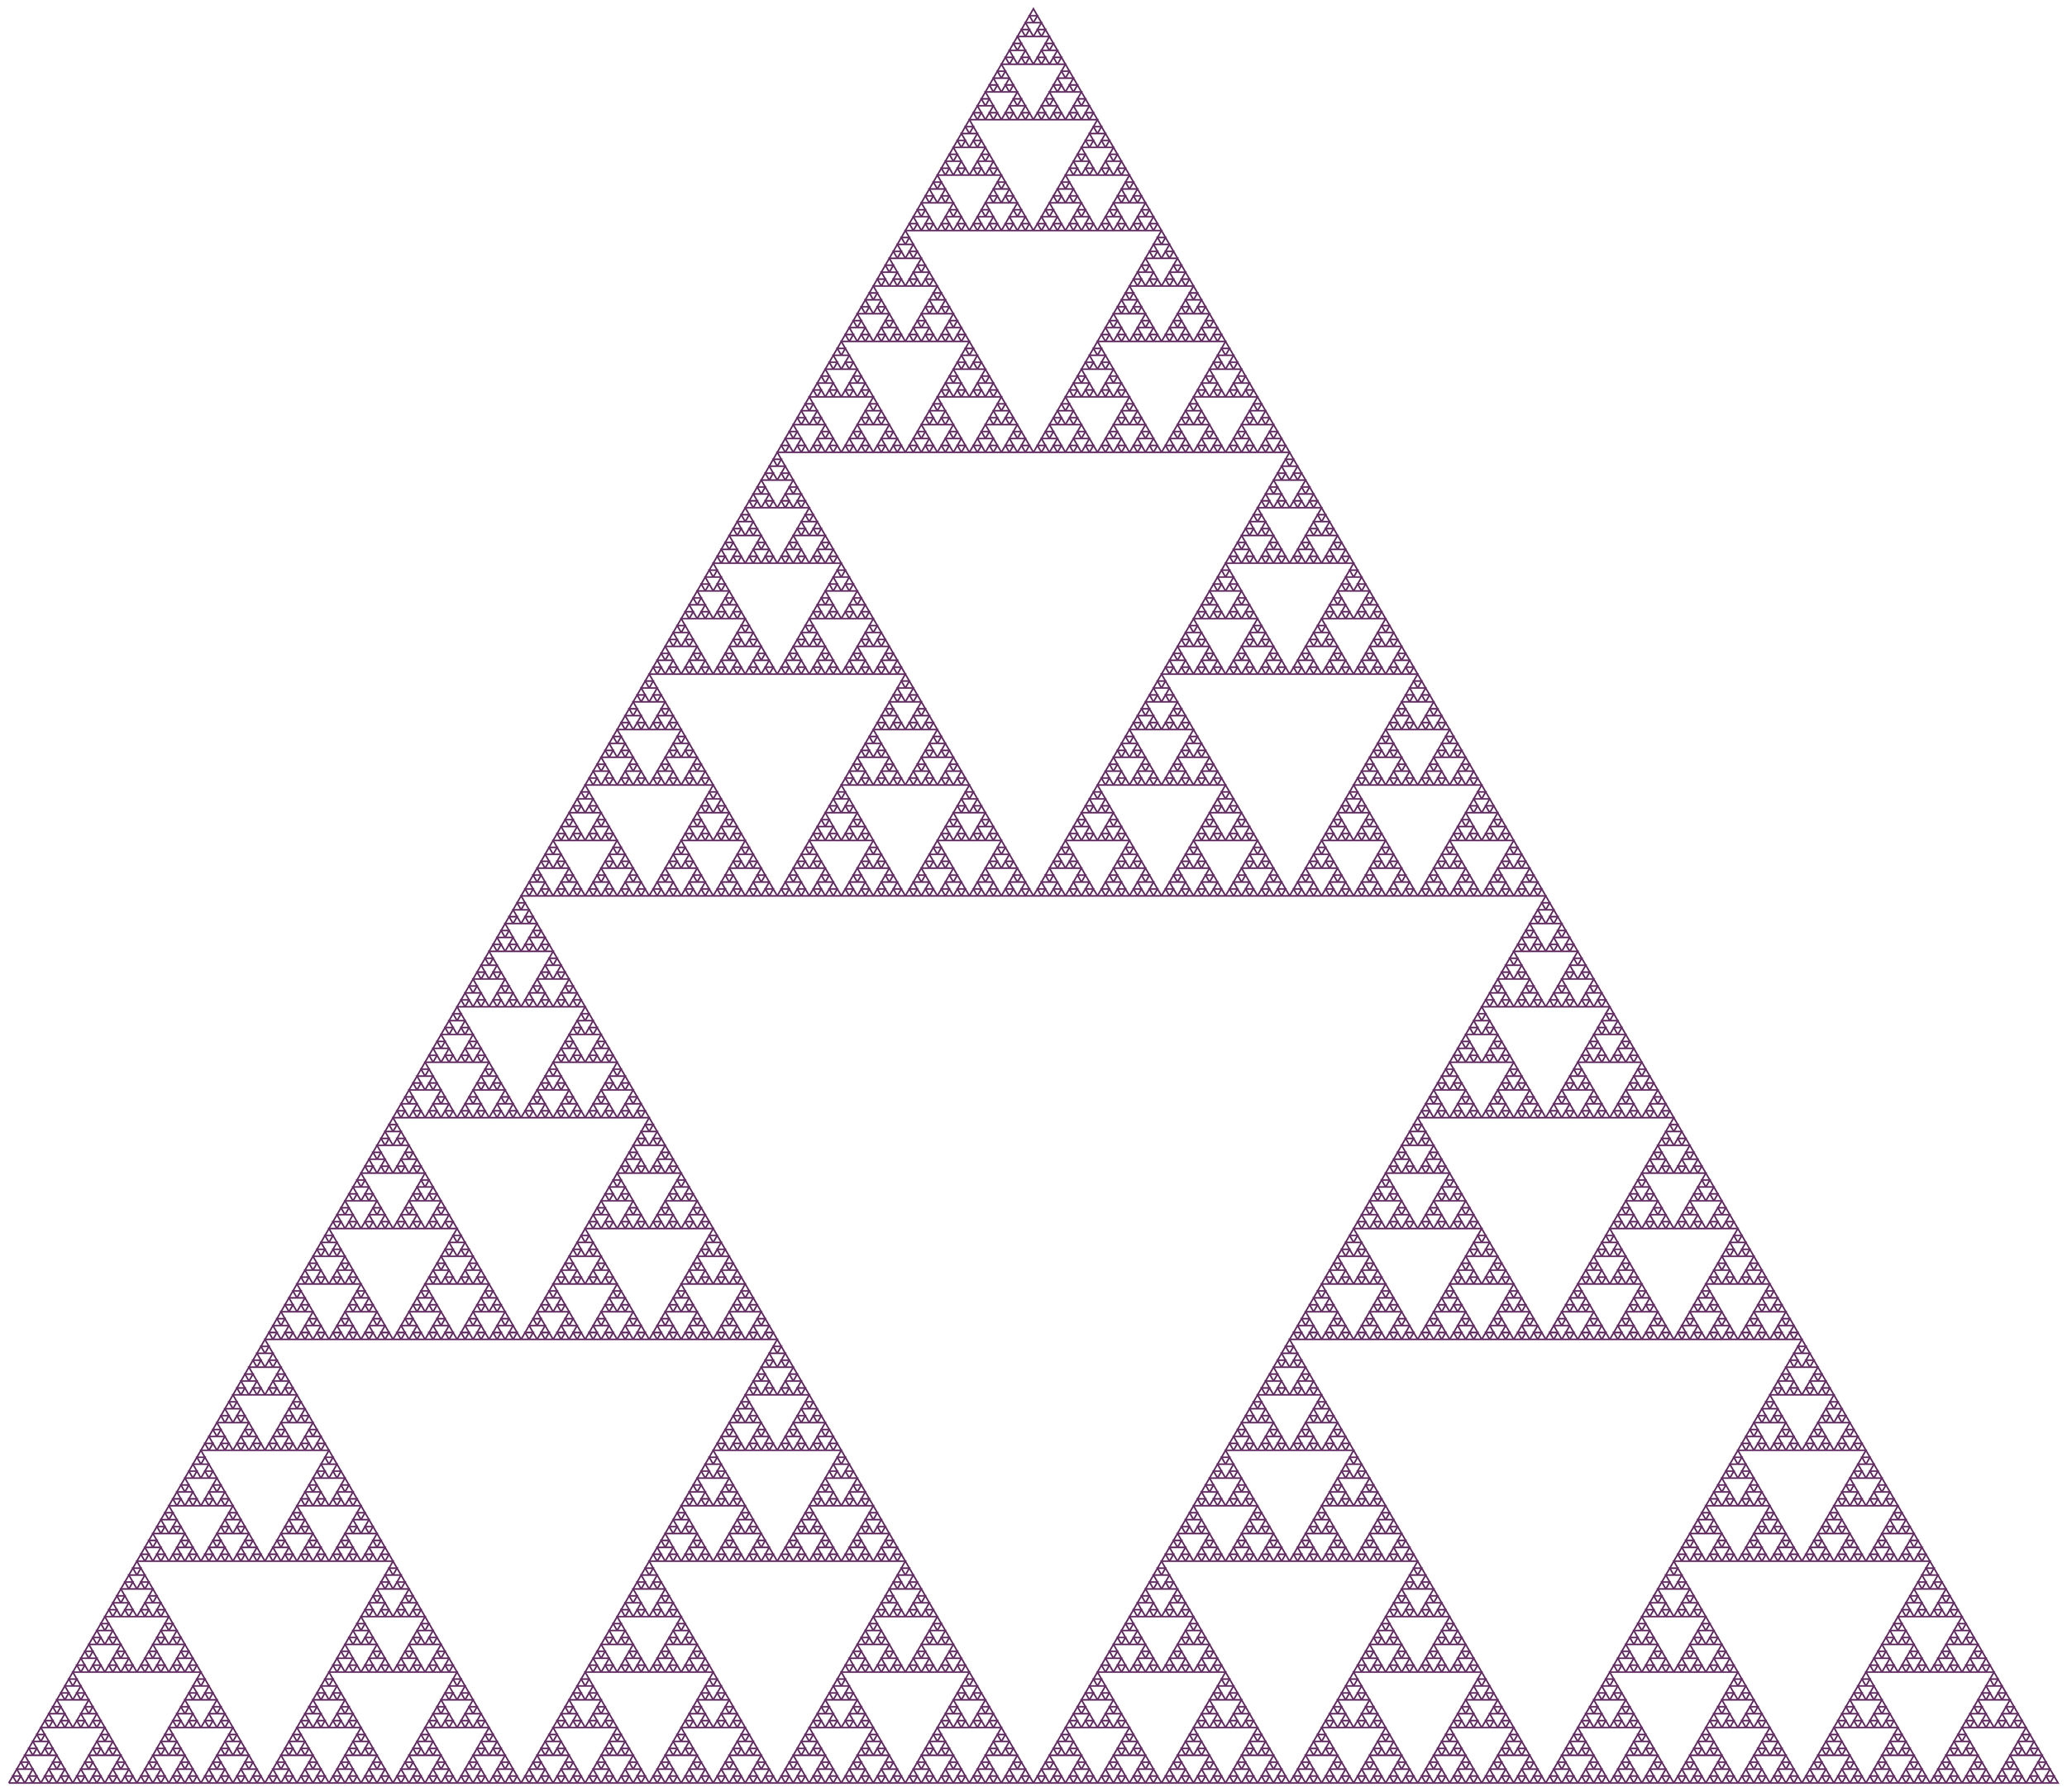
\begin{tikzpicture}
      \draw[lindenmayer system={Sierpinski Gasket, step=10, axiom=A-F-F, order=8, angle=120},pGreen,line width=2pt] lindenmayer system;
\end{tikzpicture}
\end{document}